\documentclass[ignorenonframetext,]{beamer}
\setbeamertemplate{caption}[numbered]
\setbeamertemplate{caption label separator}{: }
\setbeamercolor{caption name}{fg=normal text.fg}
\beamertemplatenavigationsymbolsempty
\usepackage{lmodern}
\usepackage{amssymb,amsmath}
\usepackage{ifxetex,ifluatex}
\usepackage{fixltx2e} % provides \textsubscript
\ifnum 0\ifxetex 1\fi\ifluatex 1\fi=0 % if pdftex
  \usepackage[T1]{fontenc}
  \usepackage[utf8]{inputenc}
\else % if luatex or xelatex
  \ifxetex
    \usepackage{mathspec}
  \else
    \usepackage{fontspec}
  \fi
  \defaultfontfeatures{Ligatures=TeX,Scale=MatchLowercase}
\fi
\usetheme[]{metropolis}
% use upquote if available, for straight quotes in verbatim environments
\IfFileExists{upquote.sty}{\usepackage{upquote}}{}
% use microtype if available
\IfFileExists{microtype.sty}{%
\usepackage{microtype}
\UseMicrotypeSet[protrusion]{basicmath} % disable protrusion for tt fonts
}{}
\newif\ifbibliography
\hypersetup{
            pdftitle={Joining dataframes in R using dplyr},
            pdfauthor={Erika Braithwaite, PhD},
            pdfborder={0 0 0},
            breaklinks=true}
\urlstyle{same}  % don't use monospace font for urls
\usepackage{color}
\usepackage{fancyvrb}
\newcommand{\VerbBar}{|}
\newcommand{\VERB}{\Verb[commandchars=\\\{\}]}
\DefineVerbatimEnvironment{Highlighting}{Verbatim}{commandchars=\\\{\}}
% Add ',fontsize=\small' for more characters per line
\usepackage{framed}
\definecolor{shadecolor}{RGB}{248,248,248}
\newenvironment{Shaded}{\begin{snugshade}}{\end{snugshade}}
\newcommand{\KeywordTok}[1]{\textcolor[rgb]{0.13,0.29,0.53}{\textbf{#1}}}
\newcommand{\DataTypeTok}[1]{\textcolor[rgb]{0.13,0.29,0.53}{#1}}
\newcommand{\DecValTok}[1]{\textcolor[rgb]{0.00,0.00,0.81}{#1}}
\newcommand{\BaseNTok}[1]{\textcolor[rgb]{0.00,0.00,0.81}{#1}}
\newcommand{\FloatTok}[1]{\textcolor[rgb]{0.00,0.00,0.81}{#1}}
\newcommand{\ConstantTok}[1]{\textcolor[rgb]{0.00,0.00,0.00}{#1}}
\newcommand{\CharTok}[1]{\textcolor[rgb]{0.31,0.60,0.02}{#1}}
\newcommand{\SpecialCharTok}[1]{\textcolor[rgb]{0.00,0.00,0.00}{#1}}
\newcommand{\StringTok}[1]{\textcolor[rgb]{0.31,0.60,0.02}{#1}}
\newcommand{\VerbatimStringTok}[1]{\textcolor[rgb]{0.31,0.60,0.02}{#1}}
\newcommand{\SpecialStringTok}[1]{\textcolor[rgb]{0.31,0.60,0.02}{#1}}
\newcommand{\ImportTok}[1]{#1}
\newcommand{\CommentTok}[1]{\textcolor[rgb]{0.56,0.35,0.01}{\textit{#1}}}
\newcommand{\DocumentationTok}[1]{\textcolor[rgb]{0.56,0.35,0.01}{\textbf{\textit{#1}}}}
\newcommand{\AnnotationTok}[1]{\textcolor[rgb]{0.56,0.35,0.01}{\textbf{\textit{#1}}}}
\newcommand{\CommentVarTok}[1]{\textcolor[rgb]{0.56,0.35,0.01}{\textbf{\textit{#1}}}}
\newcommand{\OtherTok}[1]{\textcolor[rgb]{0.56,0.35,0.01}{#1}}
\newcommand{\FunctionTok}[1]{\textcolor[rgb]{0.00,0.00,0.00}{#1}}
\newcommand{\VariableTok}[1]{\textcolor[rgb]{0.00,0.00,0.00}{#1}}
\newcommand{\ControlFlowTok}[1]{\textcolor[rgb]{0.13,0.29,0.53}{\textbf{#1}}}
\newcommand{\OperatorTok}[1]{\textcolor[rgb]{0.81,0.36,0.00}{\textbf{#1}}}
\newcommand{\BuiltInTok}[1]{#1}
\newcommand{\ExtensionTok}[1]{#1}
\newcommand{\PreprocessorTok}[1]{\textcolor[rgb]{0.56,0.35,0.01}{\textit{#1}}}
\newcommand{\AttributeTok}[1]{\textcolor[rgb]{0.77,0.63,0.00}{#1}}
\newcommand{\RegionMarkerTok}[1]{#1}
\newcommand{\InformationTok}[1]{\textcolor[rgb]{0.56,0.35,0.01}{\textbf{\textit{#1}}}}
\newcommand{\WarningTok}[1]{\textcolor[rgb]{0.56,0.35,0.01}{\textbf{\textit{#1}}}}
\newcommand{\AlertTok}[1]{\textcolor[rgb]{0.94,0.16,0.16}{#1}}
\newcommand{\ErrorTok}[1]{\textcolor[rgb]{0.64,0.00,0.00}{\textbf{#1}}}
\newcommand{\NormalTok}[1]{#1}
\usepackage{graphicx,grffile}
\makeatletter
\def\maxwidth{\ifdim\Gin@nat@width>\linewidth\linewidth\else\Gin@nat@width\fi}
\def\maxheight{\ifdim\Gin@nat@height>\textheight0.8\textheight\else\Gin@nat@height\fi}
\makeatother
% Scale images if necessary, so that they will not overflow the page
% margins by default, and it is still possible to overwrite the defaults
% using explicit options in \includegraphics[width, height, ...]{}
\setkeys{Gin}{width=\maxwidth,height=\maxheight,keepaspectratio}

% Prevent slide breaks in the middle of a paragraph:
\widowpenalties 1 10000
\raggedbottom

\AtBeginPart{
  \let\insertpartnumber\relax
  \let\partname\relax
  \frame{\partpage}
}
\AtBeginSection{
  \ifbibliography
  \else
    \let\insertsectionnumber\relax
    \let\sectionname\relax
    \frame{\sectionpage}
  \fi
}
\AtBeginSubsection{
  \let\insertsubsectionnumber\relax
  \let\subsectionname\relax
  \frame{\subsectionpage}
}

\setlength{\parindent}{0pt}
\setlength{\parskip}{6pt plus 2pt minus 1pt}
\setlength{\emergencystretch}{3em}  % prevent overfull lines
\providecommand{\tightlist}{%
  \setlength{\itemsep}{0pt}\setlength{\parskip}{0pt}}
\setcounter{secnumdepth}{0}
\usepackage{tikz}
\usepackage{pgfplots}
\usepackage{graphicx}
\usepackage{bm}
\usepackage{amsmath}
\usepackage{amssymb}
\usepackage{mathtools}
\usetikzlibrary{shadows,shapes,arrows,automata,calc,shapes.geometric,shapes.multipart,positioning,trees}

\title{Joining dataframes in R using dplyr}
\subtitle{RLadies Montreal}
\author{Erika Braithwaite, PhD}
\date{March 15, 2018}

\begin{document}
\frame{\titlepage}

\begin{frame}[fragile]{What is joining?}

We often run into scenarios where we need to join two dataframes
together. Let's say we had some students who were given an IQ test at a
career fair. Some of the students showed up at on both days, but not
all. They were given unique alphanumeric identifiers.

Set up

\begin{Shaded}
\begin{Highlighting}[]
\CommentTok{#install.packages('pacman')}
\NormalTok{pacman}\OperatorTok{::}\KeywordTok{p_load}\NormalTok{(knitr, kableExtra, formattable, data.table, dplyr, }
\NormalTok{               rmarkdown, magrittr)}
\end{Highlighting}
\end{Shaded}

Make some data

\begin{Shaded}
\begin{Highlighting}[]
\NormalTok{day1 =}\StringTok{  }\KeywordTok{data.table}\NormalTok{(}\DataTypeTok{ID=}\NormalTok{LETTERS[}\DecValTok{1}\OperatorTok{:}\DecValTok{12}\NormalTok{],}
                 \DataTypeTok{IQ=}\KeywordTok{round}\NormalTok{(}\KeywordTok{rnorm}\NormalTok{(}\DecValTok{12}\NormalTok{, }\DecValTok{100}\NormalTok{, }\DecValTok{15}\NormalTok{),}\DecValTok{2}\NormalTok{))}

\NormalTok{day2 =}\StringTok{  }\KeywordTok{data.table}\NormalTok{(}\DataTypeTok{ID=}\NormalTok{LETTERS[}\DecValTok{6}\OperatorTok{:}\DecValTok{17}\NormalTok{],}
                 \DataTypeTok{IQ=}\KeywordTok{round}\NormalTok{(}\KeywordTok{rnorm}\NormalTok{(}\DecValTok{12}\NormalTok{, }\DecValTok{100}\NormalTok{, }\DecValTok{20}\NormalTok{),}\DecValTok{2}\NormalTok{))}
\end{Highlighting}
\end{Shaded}

There are 12 individuals on day 1 and 12 individuals on day 2. 17 people
have a single measurement while 5 have 2 measurements.

\end{frame}

\begin{frame}{Our data}

ID

IQ

A

83.99

B

116.49

C

89.10

D

106.22

E

113.41

F

118.04

G

100.00

H

102.54

I

95.26

J

97.08

K

110.38

L

96.49

ID

IQ

F

86.15

G

92.67

H

87.03

I

89.36

J

87.63

K

121.33

L

84.84

M

91.99

N

119.99

O

98.95

P

90.41

Q

111.27

Let's explore the three(ish) types of joins in dplyr

\end{frame}

\begin{frame}[fragile]{Mutating joins}

\begin{block}{Mutating join: \textbf{add a new variables} to one table
from matching rows in another}

\begin{itemize}
\tightlist
\item
  \texttt{left\_join}: prioritizes left df
\item
  \texttt{right\_join}: prioritizes righ df
\item
  \texttt{inner\_join}: only retains rows in both dfs
\item
  \texttt{full\_join}: retains all rows
\end{itemize}

\end{block}

\end{frame}

\begin{frame}[fragile]{Filtering joins}

\begin{block}{Filtering join: \textbf{filter observations} from the
primary based on whether they are present in the secondary table}

\begin{itemize}
\tightlist
\item
  \texttt{semi\_join}: retains rows in the primary table that are also
  present in secondary table
\item
  \texttt{anti\_join}: retains rows in the primary that are not present
  in the secondary table
\end{itemize}

\end{block}

\end{frame}

\begin{frame}[fragile]{Set operations}

\begin{block}{Set}

\begin{itemize}
\tightlist
\item
  \texttt{intersect}:
\item
  \texttt{union}:
\item
  \texttt{setdiff}:
\end{itemize}

\end{block}

\end{frame}

\begin{frame}[fragile]{Main arguments}

\begin{Shaded}
\begin{Highlighting}[]
\KeywordTok{right_join}\NormalTok{(x, y, }\DataTypeTok{by =} \OtherTok{NULL}\NormalTok{, }\DataTypeTok{copy =} \OtherTok{FALSE}\NormalTok{, }\DataTypeTok{suffix =} \KeywordTok{c}\NormalTok{(}\StringTok{'.x'}\NormalTok{, }\StringTok{'.y'}\NormalTok{), ...)}
\end{Highlighting}
\end{Shaded}

X and Y are the two dataframes we are joining by = key variable
(typically a unique identifier). + primary key: unique in at table in
the primary table which can be one or several columns + foreign key: the
second table, which will be matched to the primary tables based on the
primary key.

copy = suffix = R will add a suffix to columns when they have the same
name

\end{frame}

\begin{frame}{Mutating joins}

\begin{figure}
\centering
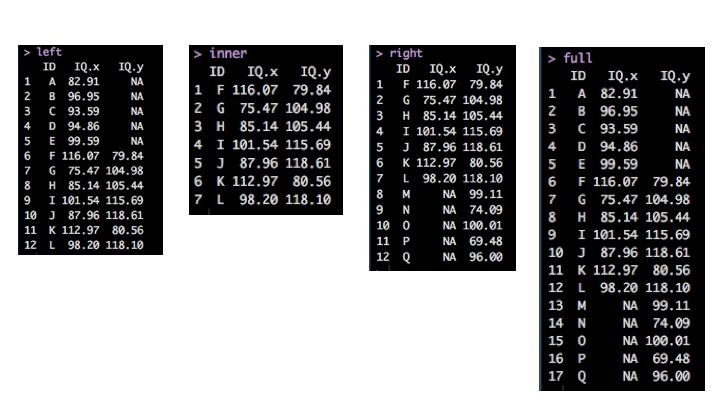
\includegraphics{graphs/mutate.png}
\caption{}
\end{figure}

\end{frame}

\begin{frame}{Filtering joins}

\begin{figure}
\centering
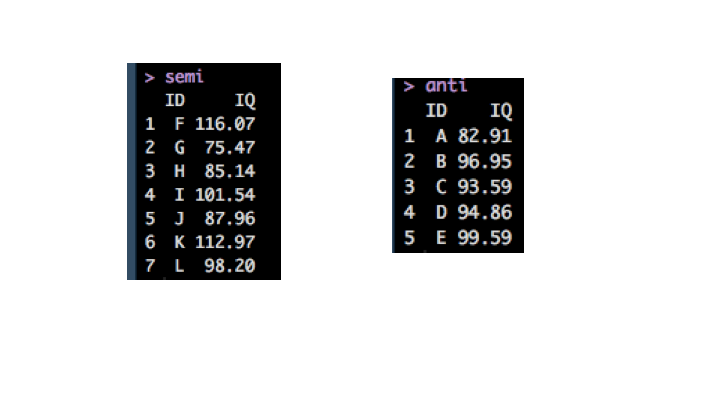
\includegraphics{graphs/filter.png}
\caption{}
\end{figure}

\end{frame}

\begin{frame}{Set operations}

\begin{figure}
\centering
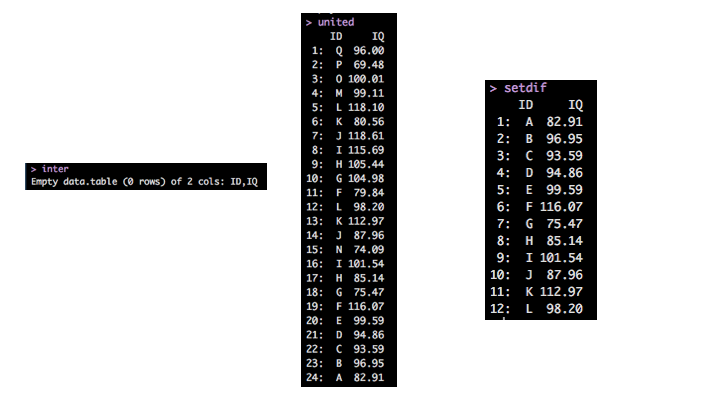
\includegraphics{graphs/set.png}
\caption{}
\end{figure}

\end{frame}

\begin{frame}[fragile]{dplyr versus data.table versus base R}

\begin{block}{Base R}

\begin{Shaded}
\begin{Highlighting}[]
\KeywordTok{rbind}\NormalTok{(...,}\DataTypeTok{use.names =}\NormalTok{ T, }\DataTypeTok{fill =}\NormalTok{ F, }\DataTypeTok{idcol =} \OtherTok{NULL}\NormalTok{)}
\end{Highlighting}
\end{Shaded}

\texttt{merge}, \texttt{rbind}, and \texttt{cdind} * Slower than dplyr *
Can't handle lists of dataframes * \texttt{rbind} returns an error when
columns are not identical * \texttt{.id} arguments allows you to specify
a name for each source dataframe

\end{block}

\begin{block}{Base R}

\begin{Shaded}
\begin{Highlighting}[]
\KeywordTok{merge}\NormalTok{(x, y, }\DataTypeTok{by =} \KeywordTok{intersect}\NormalTok{(}\KeywordTok{names}\NormalTok{(x), }\KeywordTok{names}\NormalTok{(y)),}
      \DataTypeTok{by.x =}\NormalTok{ by, }\DataTypeTok{by.y =}\NormalTok{ by, }\DataTypeTok{all =} \OtherTok{FALSE}\NormalTok{, }\DataTypeTok{all.x =}\NormalTok{ all, }\DataTypeTok{all.y =}\NormalTok{ all,}
      \DataTypeTok{sort =} \OtherTok{TRUE}\NormalTok{, }\DataTypeTok{suffixes =} \KeywordTok{c}\NormalTok{(}\StringTok{".x"}\NormalTok{,}\StringTok{".y"}\NormalTok{), }\DataTypeTok{no.dups =} \OtherTok{TRUE}\NormalTok{,}
      \DataTypeTok{incomparables =} \OtherTok{NULL}\NormalTok{, ...)}
\end{Highlighting}
\end{Shaded}

\end{block}

\begin{block}{Data.table}

\begin{Shaded}
\begin{Highlighting}[]
\KeywordTok{cbind}\NormalTok{()}
\end{Highlighting}
\end{Shaded}

\begin{verbatim}
## NULL
\end{verbatim}

\end{block}

\end{frame}

\begin{frame}{When joining can get tricky\ldots{}}

\begin{itemize}
\item
  Joining with columns having the same name but different encoding
  (UTF-8 vs.~Latin)
\item
  Joining with columns having different storage types (factors,
  integers, bit64, dates)
\item
\end{itemize}

\end{frame}

\begin{frame}{How to choose?}

Dplyr has come a long way in terms of speed. Recent benchmarking
conducted in Stack Overflow showed that dplyr starts to substantially
lag when there are a large number of groups (\textgreater{}100k).

While this point is contentious, if you've been a long standing
tidyversalist, then you might find data.table's syntax more difficult to
learn.

\end{frame}

\begin{frame}{More!}

There are additional types of joins not covered here: rolling joins,
scaling joins

Rolling joins are used in circumstances where you want to map a
dataframe to another based but you lack a common ID e.g.~merging
observations based on logical arguments.

Resources

\end{frame}

\begin{frame}{Thank-you}

\end{frame}

\end{document}
